\documentclass[12pt]{article}
\usepackage[margin=0.7in]{geometry} 		% defines page margin
\usepackage{knitting} 				% defines \chart and \textknit
\usepackage{titling} 				% title page
\usepackage{graphicx,xspace, scrextend, moresize, enumitem}	% defines space control stuff
\usepackage{tabularx, array, colortbl}	% defines tables
\usepackage{multicol} 				% defines columns
\usepackage{multirow} 				% defines multirows, combined cells in tables
\usepackage{framed, mdframed} 				% defines boxes for notes and written directions
\usepackage[x11names]{xcolor} 		% extends color library
\pdfmapfile{+knitfont.map}

% font selection
\usepackage{palatino, moresize, sectsty}
\allsectionsfont{\sffamily}

\renewcommand{\arraystretch}{2}

\newcolumntype{L}[1]{>{\leftalign\arraybackslash}p{#1}}
\newcolumntype{C}[1]{>{\centering\arraybackslash}p{#1}}

% length parameters
\setlength{\parindent}{0pt} % disables indentation for paragraphs
\setlength{\columnsep}{0.7cm} % column separation in multicol environment

% color parameters
\colorlet{framecolor}{black}
\colorlet{shadecolor}{LemonChiffon1}
\colorlet{highlight}{yellow}
\colorlet{purlgray}{black}
\colorlet{knittext}{black}

\renewcommand{\purlboxbackground}{\color{purlgray}}

\newcommand{\FG}[1]{{\color{white} \Purl{#1}{#1}}}
\newcommand{\BG}[1]{{\color{black} \Knit{#1}{#1}}}

% custom commands
\newcommand{\comment}[1]{} % allows for multiline comments that LaTeX will ignore

\newcommand{\vocab}[1]{\emph{\textbf{#1}}} % format for highlighting definitions of stitches, vocabulary terms
\newcommand{\rowDir}[1]{\textbf{#1:}} % indent for written instructions within paragraphs

\renewcommand{\repeat}[1]{\textbf{*[#1]*}} % format for written repeats, bold with *[ stitches ]*

\newcommand{\increase}[1]{(\emph{+#1 
	\ifnum#1=1{st}\else{sts}\fi})}
\newcommand{\decrease}[1]{(\emph{$-$#1
	\ifnum#1=1{st}\else{sts}\fi})}
\newcommand{\stitchcount}[1]{(\emph{#1 sts})}

\newcommand{\rnfive}{\rnright\addtocounter{rownumber}{-4}} % used when numbering every fifth row in a chart


% thick horizontal line
\makeatletter \newcommand{\thickhline}{
    \noalign {\ifnum 0=`}\fi \hrule height 1.5pt
    \futurelet \reserved@a \@xhline
}
\makeatother

% custom environments
\newenvironment{frnote}
    {% framed environment for pattern notes
    	\setlength{\FrameRule}{1.5pt}
    	\def\FrameCommand{\fboxrule=\FrameRule\fboxsep=\FrameSep \fcolorbox{framecolor}{shadecolor}}
    	\MakeFramed {\FrameRestore}}
    {\setlength{\FrameRule}{1pt}
	\endMakeFramed}

\newenvironment{frdirection}
    {% framed environment for written directions
	\def\FrameCommand{\fboxrule=\FrameRule\fboxsep=\FrameSep \fbox}
   	\MakeFramed {\advance\hsize-\width \FrameRestore}
    	\addmargin[1.5cm]{0pt}}
    {\endaddmargin
	\endMakeFramed}

\newenvironment{unframed}
    {% unframed environment for written directions
	\begin{addmargin}[2em]{0pt}
	}
    {
	\setlength{\parindent}{0em}
	\end{addmargin}}

\title{Helicase Scarf}
\author{Shanel Wu (Piper Nell)}

\begin{document}

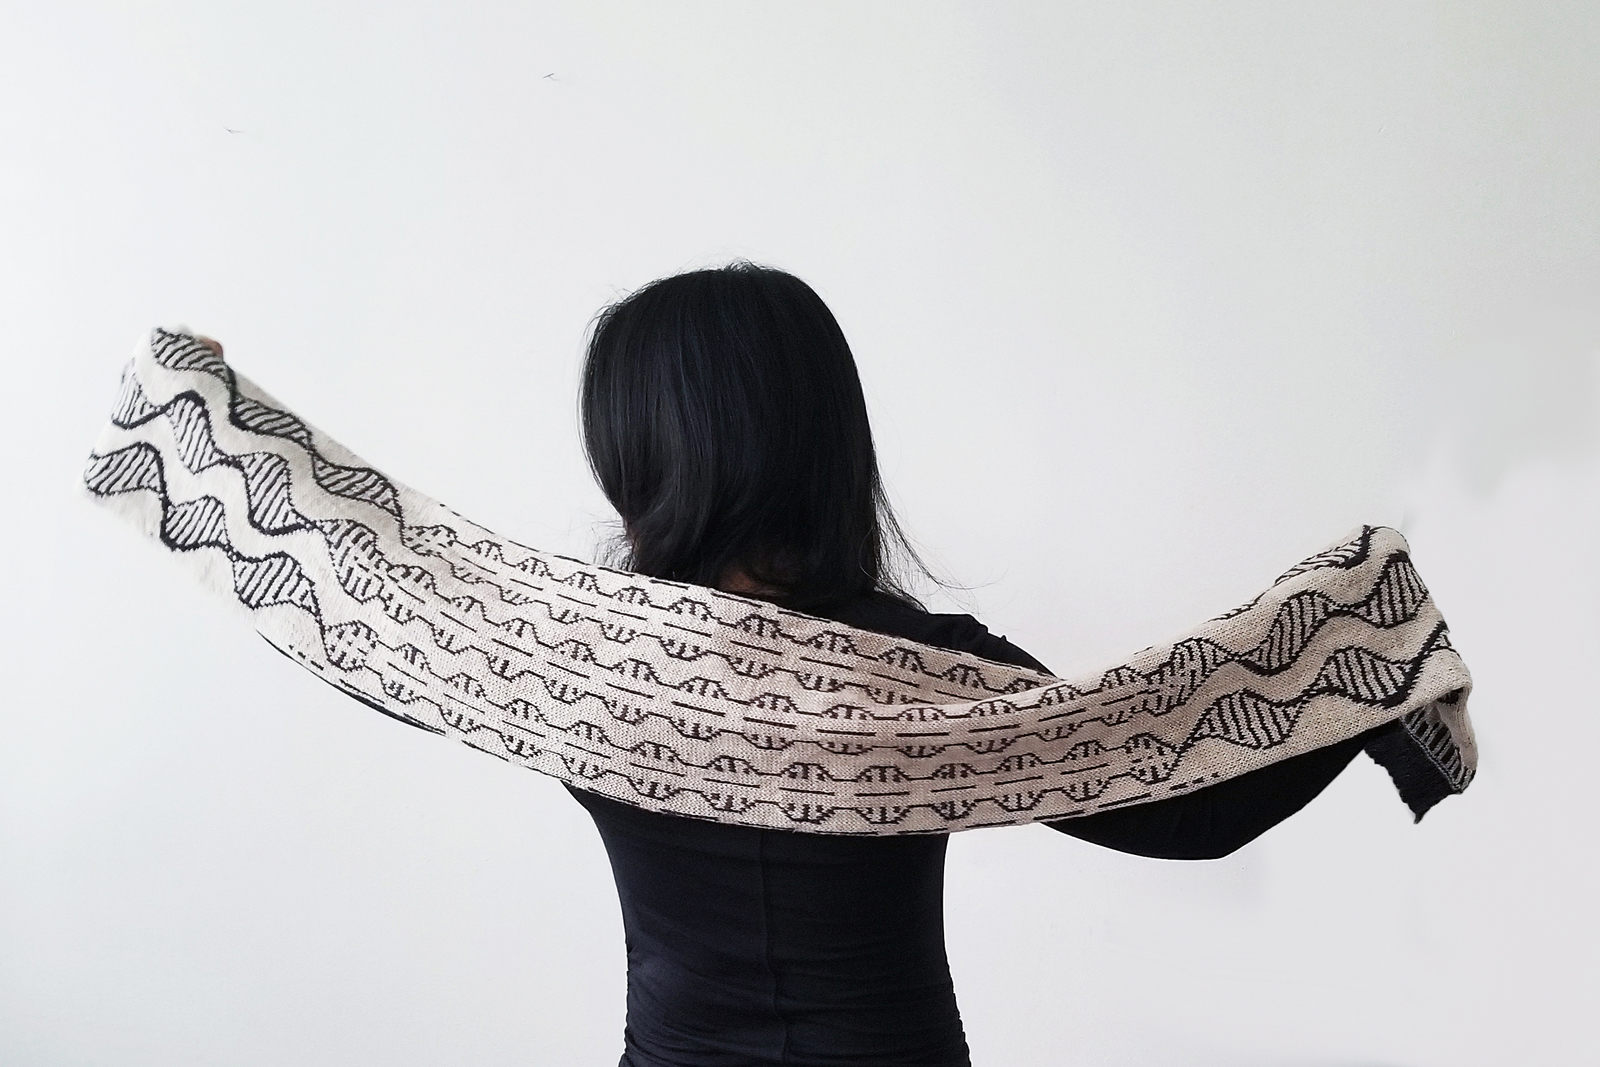
\includegraphics[width=\linewidth]{spread-small.jpg}
\vspace{1em}

{\fontfamily{qag}\selectfont
\HUGE\textbf{\thetitle}
\hspace{3em} % adjust this space
\normalsize\theauthor
}

\small
\begin{multicols}{2}
% TODO: description here
Helicase is the protein that ``unzips" and re-zips DNA molecules, enabling life as we know it to function. Through the magic of stranded knitting, you too can unzip and re-zip strands of DNA!

\subsubsection*{Techniques}

This pattern is written for an advanced knitter experienced with stranded colorwork and reading charts. You will have to work extensively from charts, and even read them upside-down (i.e. top-to-bottom rather than bottom-to-top). 

\vspace{1em}
You will also have to catch many long floats. Catch floats by twisting the two working yarns every 6 to 8 stitches, but don't worry too much about long floats as they will all be inside the work once the scarf is complete. To minimize the number of floats you catch, you need to be comfortable leaving floats as long as 7 or 8 stitches.

\vfill
\columnbreak

\subsubsection*{Yarn Requirements}

Fingering weight yarn in 2 highly contrasting colors, C1 \& C2. Two 100g/400y skeins of each color. 

\vspace{1em}
\emph{Sample used Pancake and Lulu PLY Twist Fingering in ``bone" as C1 and Sparkle Fingering in ``charcoal". 195g/780y of C1 and 140g/620y of C2.}

\subsubsection*{Sizing/Gauge}
41 sts x 31 rows = 4" in stockinette stitch. Sample measures 62" long and 7.5" wide.

\subsubsection*{Tools}
\begin{itemize}
\item 16" circular needle in size US2/2.75mm (or size needed to obtain gauge) for colorwork
\item Additional needle (circular or straight) in the same size for ribbing
\item Two stitch markers in different colors
\end{itemize}

\end{multicols}
\begin{multicols}{2}
\small

\subsection*{Pattern Key}

% stitch key - fill in with all stitches used in design: chart symbol, written abbreviation, full stitch name or explanation
% stitches with explanations must first be BOLDED, followed by colon then explanation
\renewcommand{\arraystretch}{1.3}
\begin{tabular}{| C{0.2\linewidth}  p{0.6\linewidth} | }
\thickhline \rowcolor{shadecolor} 
\textbf{Abbr.}	& \textbf{Description} \\ \thickhline
C1	& Color 1 \\
C2	& Color 2 \\
pm	& place marker \\
sm	& slip marker \\
CO	& cast on \\
k	&  knit \\
p	& purl   \\
\hline
\end{tabular}

\vfill
\columnbreak

\section*{Cast On and Set Up}

With the Long Tail Cast On, use C1 to CO 130 sts. Pm for beginning of round and join in the round. Work the following two rounds once.
\\
\begin{unframed}
\rowDir{Rnd 1} K 65 sts in C1, then pm (with different color marker) to mark halfway point of the round. K to end of round, sm.

\rowDir{Rnd 2} K one more round of stockinette in C1. At the end of the second round, sm, join C2, and begin working from the chart directions.
\end{unframed}

\end{multicols}

\vspace{-1em}

\small

\section*{Chart Directions}
In every chart, you will work each chart twice per round, with the markers separating each repeat.
\begin{enumerate}[itemsep=0mm]
\item Work Rnds 1-39 of Chart 1 once.
\item Work Rnds 1-60 of Chart 2 once.
\item Work Rnds 1-31 of Chart 3 once. 
\item Work Rnds 1-16 of Chart 4 for 11 repeats. % After 6 repeats a little under half of yarn used up
Work Rnds 1-5 once more to end the section.
\item Work Chart 3 from top to bottom (Rnds 31 to 1) once.
\item Work Chart 2 from top to bottom (Rnds 60 to 1) once.
\item Work Chart 1 from top to bottom (Rnds 39 to 1) once.
\item Break C2, work 1 round of stockinette in C1, then bind off in C1. Remove markers as you come to them when binding off. Weave in ends and lightly block, then proceed to ribbing directions.
\end{enumerate}

\section*{Ribbing Directions}

Your work should be a long tube with open ends. In this section, you will finish the scarf by closing the ends and working ribbed accents. You may want to divide your remaining C2 in half.

\begin{enumerate}[itemsep=0mm]
\item Starting at the old beginning of round and using C2, pick up and knit 130 sts. Do not join in the round. 
\item Fold stitches in half and place two ends of circular needle side by side as if working a three-needle bind-off. In this step, you will be using your 3rd needle to k2a and p2a (``a" as in ``across needles") as follows:
\begin{unframed}
\small
\vocab{k2a} - insert 3rd needle knitwise into both 1st st on needle 1 and 1st st on needle 2. K2tog. \\
\vocab{p2a} - insert 3rd needle purlwise into both 1st st on needle 1 and 1st st on needle 2. P2tog.
\end{unframed}

Repeat: \repeat{k2a $\times$ 2, p2a, k2a, p2a} to end of row. You should have 65 sts on the needle.
\item Work the following 2 rows until ribbing measures 5" or half of remaining C2 is used. 
\begin{unframed}
\rowDir{Row 1} \repeat{k1, p1, k1, p2} to end of row \\
\rowDir{Row 2} \repeat{k2, p1, k1, p1} to end of row
\end{unframed}

\item Bind off in pattern.
\end{enumerate}

Repeat on other end of scarf. Weave in your ends and your scarf is ready to wear!

\newpage

\begin{frnote}
\textbf{Modification Suggestions} 
\begin{itemize}
\item \emph{To lengthen the scarf:} Either work additional repeats of Chart 2 or Chart 4 in Step 2, 4, or 6.
\item \emph{To shorten the scarf:} a) You can omit Chart 2 in Step 2 or 6 if you are sick of long floats. This is possible because the last round of Chart 1 can also flow straight into the first round of Chart 3. b) Work fewer repeats of Chart 4 in Step 4.
\item \emph{To use up all of your yarn:} the easiest way to maximize your yarn mileage is to modify the number of repeats of Chart 4 in Step 4. Work $n$ repeats of Chart 4 until half of C1 is used up. Then work $n-1$ repeats of Chart 4 to finish the section and continue with the rest of the scarf.
\end{itemize}
\end{frnote}

%%%%%%%%%%%%%%%%%%%%%%%%%%%%%%%%%%%%%%%%%%%%%%%%%
\section*{Charts}

\colorlet{knitlinecolor}{yellow}
\hspace{2em} \chart{-} C1 \hspace{1em} \chart{=} C2

\centering
\subsection*{Chart 1: Telomeres} 

\tiny
\chart{
--==\BG{16}=\BG{10}=-===------==\BG{16}=---- \rnright \addtocounter{rownumber}{-3}
---==\BG{15}=\BG{10}==-===------==\BG{15}=----
----==-\FG{14}\BG{10}=---===------==-\FG{14}----
-----==\BG{13}=\BG{10}=----===------==\BG{13}=----
\overline*{------==\BG{12}=\BG{9}=-====-===------==\BG{12}=----} \rnfive

-------==-\FG{10}\BG{10}=-------===------==-\FG{10}-----
--------==\BG{9}=\BG{9}=\BG{9}==-------==\BG{9}=-----
\BG{9}==-------=\BG{9}=-\FG{12}-------==-------=------
\BG{9}==-====-=\BG{9}=\BG{12}==-------==-====-=-------
\overline*{\BG{10}==----=\BG{9}=\BG{13}==--------==----=--------} \rnfive

\BG{10}==---=\BG{9}=-\FG{15}--------==---=\BG{9}
\BG{10}===-=\BG{9}=\BG{15}==--------===-=\BG{10}
\BG{10}==-=\BG{9}=\BG{16}==--------==-=\BG{11}
\BG{10}===\BG{10}\FG{18}\BG{9}===\BG{12}
\overline*{\BG{9}==-=\BG{9}=\BG{16}==--------==-=\BG{12}} \rnfive

\BG{9}===\BG{10}=\BG{15}==\BG{9}===\BG{13}
--------==-=\BG{10}\FG{14}-==\BG{9}==-=\BG{13}
--------=-==\BG{10}=\BG{13}==\BG{10}=-==\BG{13}
-------=--==\BG{10}=\BG{12}==\BG{10}=--==\BG{13}
\overline*{------=---==\BG{11}\FG{10}-==\BG{10}=---==\BG{13}} \rnfive

-----=-======\BG{10}=\BG{9}==\BG{10}=-======\BG{12}
----=------==\BG{10}=\BG{9}==\BG{9}=------==\BG{12}
---=--------== \BG{9} ==  -----  -=-==  -------- =--------== \BG{11}
---\FG{12}  -----  ---==  -----  -=-==  ----- ---\FG{12}  \BG{10}
\overline*{---=\Knit{9}{9}==  -----  ---==  -=-==  -=-==  ----- ---=\Knit{9}{9}==  \Knit{10}{10}} \rnfive

---=\Knit{9}{9}==  -----  ---==  -=-==  -=-==  ----- ---=\Knit{9}{9}==  \Knit{10}{10}
---== 	 -----  -=-==  -----  ---==  -=-==  -=-==  -----  ---==  -----  -=-==  \Knit{10}{10}
---== 	 -----  -=-==  -----  ---==  -=-==  -=-==  -----  ---==  -----  -=-==  \Knit{10}{10}
-=-==  -=-==  -=-==  -=---  -=-==  -=-==  -=-==  -=---  -=-==  -=-==  -=-==  -=---  -=---
\overline{-=-==  -=-==  -=-==  -=---  -=-==  -=-==  -=-==  -=---  -=-==  -=-==  -=-==  -=---  -=---} \rnfive

-=-==  -=-==  -=-==  -=-==  -=-==  -=-==  -=-==  -=-==  -=-==  -=-==  -=-==  -=-==  -=-==  
-=-==  -=-==  -=-==  -=-==  -=-==  -=-==  -=-==  -=-==  -=-==  -=-==  -=-==  -=-==  -=-==
-=-==  -=-==  -=-==  -=-==  -=-==  -=-==  -=-==  -=-==  -=-==  -=-==  -=-==  -=-==  -=-==
-=-==  -=-==  -=-==  -=-==  -=-==  -=-==  -=-==  -=-==  -=-==  -=-==  -=-==  -=-==  -=-==
\overline*{-=-==  -=-==  -=-==  -=-==  -=-==  -=-==  -=-==  -=-==  -=-==  -=-==  -=-==  -=-==  -=-==}\rnfive \addtocounter{rownumber}{1}
-----------------------------------------------------------------
=================================================================
-----------------------------------------------------------------
================================================================= \rnright
}

{
\normalsize

\newpage
\subsection*{Chart 2: Double Helix}
}

\chart{
\overline*{--==\BG{16}=\BG{10}=-===------==\BG{16}=----} \rnfive
---==\BG{15}=\BG{10}==-===------==\BG{15}=----
----==-\FG{14}\BG{10}=---===------==-\FG{14}----
-----==\BG{13}=\BG{10}=----===------==\BG{13}=----
------==\BG{12}=\BG{9}=-====-===------==\BG{12}=----
\overline*{-------==-\FG{10}\BG{10}=-------===------==-\FG{10}-----} \rnfive

--------==\BG{9}=\BG{9}=\BG{9}==-------==\BG{9}=-----
\BG{9}==-------=\BG{9}=-\FG{12}-------==-------=------
\BG{9}==-====-=\BG{9}=\BG{12}==-------==-====-=-------
\BG{10}==----=\BG{9}=\BG{13}==--------==----=--------
\overline*{\BG{10}==---=\BG{9}=-\FG{15}--------==---=\BG{9}} \rnfive

\BG{10}===-=\BG{9}=\BG{15}==--------===-=\BG{10}
\BG{10}==-=\BG{9}=\BG{16}==--------==-=\BG{11}
\BG{10}===\BG{10}\FG{18}\BG{9}===\BG{12}
\BG{9}==-=\BG{9}=\BG{16}==--------==-=\BG{12}
\overline*{\BG{9}===\BG{10}=\BG{15}==\BG{9}===\BG{13}} \rnfive

--------==-=\BG{10}\FG{14}-==\BG{9}==-=\BG{13}
\BG{8}=-==\BG{10}=\BG{13}==\BG{10}=-==\BG{13}
\BG{7}=--==\BG{10}=\BG{12}==\BG{10}=--==\BG{13}
------=---==\BG{11}\FG{10}-==\BG{10}=---==\BG{13}
\overline*{-----=-======\BG{10}=\BG{9}==\BG{10}=-======\BG{12}} \rnfive

----=------==\BG{11}=-------==\BG{10}=------==\BG{12}
---=\BG{8}==\BG{11}=-====-==\BG{9}=\BG{8}==\BG{11}
---\FG{12}\BG{11}=----==\BG{10}\FG{12}\BG{10}
--=\BG{11}==\BG{11}=---==\BG{9}=\BG{11}==\BG{9}
\overline*{--=\BG{12}==\BG{11}=-===\BG{9}=\BG{12}==\BG{8}} \rnfive

--\FG{16}\BG{11}=-==\BG{9}\FG{16}-------
--=\BG{14}==\BG{11}===\BG{9}=\BG{14}==------
--=\BG{15}==\BG{10}=-==\BG{8}=\BG{15}==-----
---\FG{17}\BG{11}===\BG{9}\FG{17}-----
\overline*{---=\BG{15}==\BG{10}=-==\BG{8}=\BG{15}==----} \rnfive

----=\BG{14}===\BG{9}==-=\BG{9}=\BG{14}===---
-----=-\FG{15}\BG{9}==--=\BG{9}=-\FG{15}---
------=\BG{12}===\BG{9}==---=\BG{9}=\BG{12}===---
-------=\BG{11}===\BG{8}======-=\BG{9}=\BG{11}===---
\overline*{\BG{8}=-\FG{12}\BG{8}==------=\BG{9}=-\FG{12}---} \rnfive

\BG{9}=\BG{8}===\BG{8}==\BG{8}=\BG{9}=\BG{8}===----
\BG{10}=------===\BG{8}\FG{12}\BG{10}=------===-----
\BG{10}=-=======\BG{8}==\BG{11}=\BG{9}=-=======------
\BG{11}=---===\BG{8}==\BG{12}=\BG{10}=---===-------
\overline*{\BG{11}=-===\BG{9}\FG{16}\BG{10}=-===\BG{9}} \rnfive

\BG{11}====\BG{9}==\BG{14}=\BG{10}====\BG{10}
\BG{11}===\BG{9}==\BG{15}=\BG{10}===\BG{11}
\BG{10}===\BG{10}\FG{17}\BG{10}===\BG{12}
\BG{9}==-=\BG{9}==\BG{15}=\BG{9}==-=\BG{12}
\overline*{\BG{8}====\BG{9}===\BG{14}=\BG{9}====\BG{13}} \rnfive

-------===-=\BG{9}\FG{15}-=\BG{9}===-=\BG{13}
------===-==\BG{9}===\BG{12}=\BG{9}===-==\BG{13}
-----===---=\BG{9}===\BG{11}=\BG{9}===---=\BG{13}
----===----=\BG{9}\FG{12}-=\BG{9}===----=\BG{13} 
\overline*{---===-====-=\BG{9}===\BG{8}=\BG{9}===-====-=\BG{12}} \rnfive

--===-------=\BG{10}===------=\BG{9}===-------=\BG{12}
--==\BG{9}=\BG{10}=======-=\BG{9}==\BG{9}=\BG{11}
-\FG{12}-=\BG{10}===---=\BG{9}\FG{12}-=\BG{10}
-==\BG{12}=\BG{11}===-=\BG{9}==\BG{12}=\BG{9}
\overline*{-==\BG{13}=\BG{11}====\BG{9}==\BG{13}=\BG{8}}  \rnfive \addtocounter{rownumber}{1}

-\FG{15}-=\BG{11}===\BG{9}\FG{15}-=------- 
-==\BG{15}=\BG{11}===--------==\BG{15}=------
-==\BG{16}=\BG{10}=-==-------==\BG{16}=-----
\underline*{--\FG{18}\BG{11}====-------\FG{18}-----} \rnright
}

\vfill

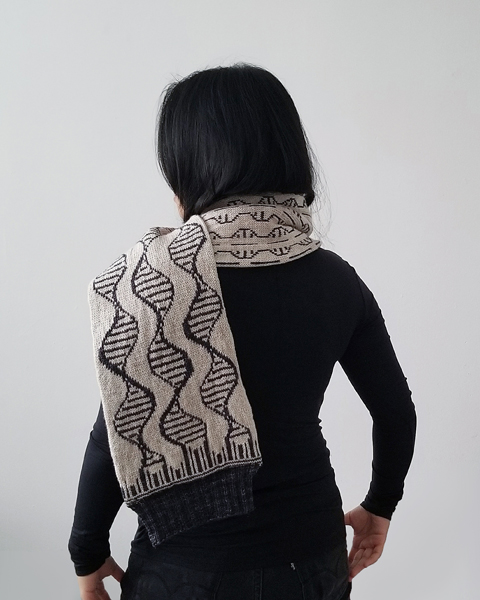
\includegraphics[height=3in]{backone-small.jpg}
\hspace{2em}
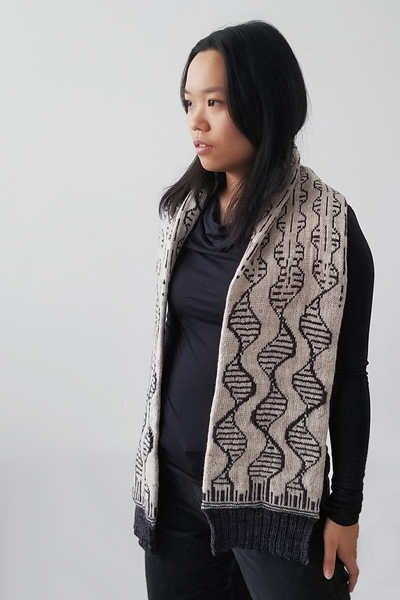
\includegraphics[height=3in]{drape-small.jpg}

% CHART 3 INSTRUCTIONS

{\normalsize
\newpage
\subsection*{Chart 3: Transition}
}

\chart{
=-----=-==----=-=-------=-==-------==-=-------=-==----=-=-----=-- \rnright

\overline*{-----=------=----=-------=-----=-----=-------=------=----=----=--} \rnfive
-----====---=--==-=-------=----=-----=-------====---=--==-=---=--
-----=\BG{13}=-------=---=--====-------=\BG{13}=-----
-----=\BG{13}=-------===--=----=-------=\BG{13}=-----
-----=-===--=--=====-------=----=-----=------=-===--=--=====-----

\overline*{=-----=\BG{12}=\BG{7}=----=------=------=\BG{12}=-----} \rnfive
=------=\BG{11}=\BG{7}====---=====-=------=\BG{11}=-----
\BG{8}=-===--==-=\BG{7}=\BG{13}=\BG{7}=-===--==-=---=--
\BG{9}=\BG{7}=\BG{8}=\BG{13}=\BG{8}=\BG{7}=----=--
=\BG{9}=-----=\BG{9}====--=--======\BG{9}=-----=-----=--

\overline*{\BG{11}==--=\BG{9}=------=\BG{7}=\BG{10}==--=\BG{9}} \rnfive
\BG{13}==\BG{9}=\BG{15}=\BG{12}==\BG{10}
\BG{12}==\BG{9}=-====--=--======\BG{12}==\BG{8}=--
=\BG{10}==\BG{9}=\BG{16}=\BG{11}==\BG{9}=--
\BG{10}=-=\BG{9}==\BG{14}=\BG{11}=-=\BG{12}

\overline*{\BG{9}===\BG{10}=-====--======-=\BG{11}===\BG{13}} \rnfive
\BG{8}==-=\BG{10}=\BG{13}=\BG{11}==-=\BG{10}=--
\BG{7}==-==\BG{10}=\BG{12}=\BG{11}==-==\BG{13}
------==---=\BG{11}\FG{10}-=\BG{11}==---=\BG{13}
-----==----=\BG{11}=\BG{9}=\BG{11}==----=\BG{13}

\overline*{----==-====-=\BG{11}=-------=\BG{11}==-====-=\BG{9}=--} \rnfive
---==-------=\BG{12}=-====-=\BG{10}==-------=\BG{12}
---=\BG{9}=\BG{12}=----=\BG{11}=\BG{9}=\BG{11}
--\FG{11}-=\BG{12}=---=\BG{10}\FG{11}-=\BG{10}
--=\BG{12}=\BG{12}=-==\BG{10}=\BG{12}=\BG{9}

\overline*{--=\BG{13}=\BG{12}=-=\BG{10}=\BG{13}=\BG{8}} \rnfive \addtocounter{rownumber}{1}
--\FG{14}-=\BG{12}==\BG{10}\FG{14}-=\BG{7}
--=\BG{15}=\BG{11}=-=\BG{9}=\BG{15}=------
--=\BG{16}=\BG{11}===\BG{8}=\BG{16}=-----
\underline*{--=-\FG{16}\BG{11}=-==\BG{7}=-\FG{16}-----} \rnright
}

% CHART 4 instructions

{\normalsize
\subsection*{Chart 4: Single Helix}
}

\chart{
=-----=----=----=-------=-==---=---==-=-------=----=----=-----=-- \rnright

\overline*{=----=-----=-----=-------=-----=-----=-------=-----=-----=----=--} \rnfive
=---=-==---=---==-=-------=----=----=-------=-==---=---==-=---=--
---=-------=-------=-------=-------=-------=-------=-------=-----
---=-------=-------=-------=-------=-------=-------=-------=-----
---=====---=---=====-------=-------=-------=====---=---=====-----

\overline*{---=-------=-------=-------=-------=-------=-------=-------=-----} \rnfive
---=-------=-------=-------=-------=-------=-------=-------=-----
=---=-==---=---==-=-------=----=----=-------=-==---=---==-=---=--
=----=-----=-----=-------=-----=-----=-------=-----=-----=----=--
=-----=----=----=-------=-==---=---==-=-------=----=----=-----=--

\overline*{=------=-------=-------=-------=-------=-------=-------=------=--} \rnfive \addtocounter{rownumber}{1}
=------=-------=-------=-------=-------=-------=-------=------=--
=------=-------=-------=====---=---=====-------=-------=------=--
=------=-------=-------=-------=-------=-------=-------=------=--
\underline*{=------=-------=-------=-------=-------=-------=-------=------=--} \rnright
}

\vfill

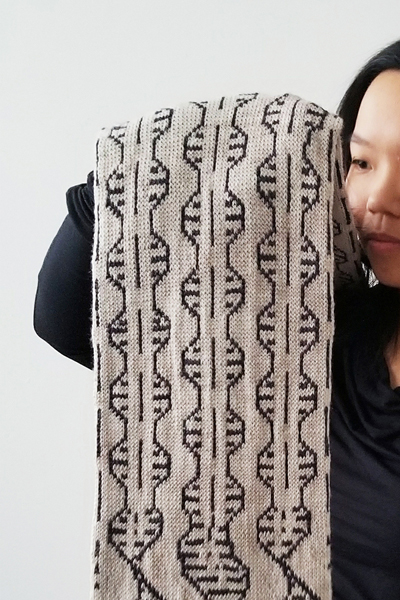
\includegraphics[height=3in]{display-small.jpg}
\hspace{2em}
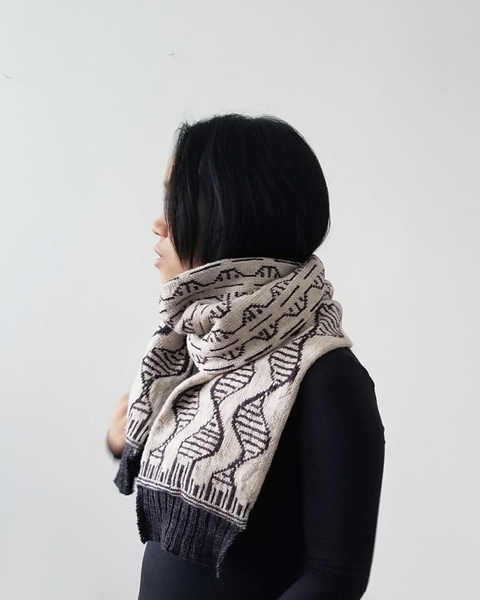
\includegraphics[height=3in]{sidetwo-small.jpg}

\vfill

\begin{flushleft}
\ssmall
Pattern and photographs \copyright 2018 Shanel Wu. All rights reserved. In purchasing this pattern, you agree to print and use this pattern only for personal use. Do not redistribute or sell paper or electronic copies of this pattern.
\end{flushleft}
\vspace{-2em}
\end{document}